\chapter{背景}
\label{chapter:background}

\section{引言}
\label{section:background:introduction}
神经科学是研究神经系统的科学研究。
神经科学的一个主要目标是理解神经系统的工作原理。
要实现这个目标,首先需要研究神经系统在各种实验条件下的表现,描述出神经系统是什么样的;
其次是研究神经系统的各种现象的生理基础,阐释出神经系统如何运行;
最后结合计算理论、信息理论等的原理,研究神经系统各种功能的意义,理解神经系统为什么这样运行。

神经科学有着多种多样的的研究方式,包括分子、细胞、环路、行为、发育、进化等研究层面。
研究中需要结合实验研究与理论模型。
模型也可以分为三个层面,描述性模型刻画出神经系统的行为,机制模型将高层次的神经系统行为与低层次的生物基础联系起来,解释性模型研究神经系统功能对认知和行为的意义\cite{Dayan2001}。

为了研究神经元细胞的特性对神经元网络的影响,就要建立神经元模型,进而组成神经元网络进行研究。

\section{神经系统}
\label{section:background:neuron-model}
神经元是神经系统的最基本的信息处理单元,它们之间通过突触连接起来。
图\ref{figure:cajal-nerve-cells}是 Ramón y Cajal 绘制的猫的肠肌层中的神经元细胞\cite{Cajal1909},图中两个神经元细胞体的位置有字母标出,由细胞体发出的线状的结构是树突和轴突。
Ramón y Cajal 也因为对神经系统结构的研究与 Camillo Golgi 共同获得了1906年的诺贝尔生理学或医学奖。

\begin{figure}
  \centering
  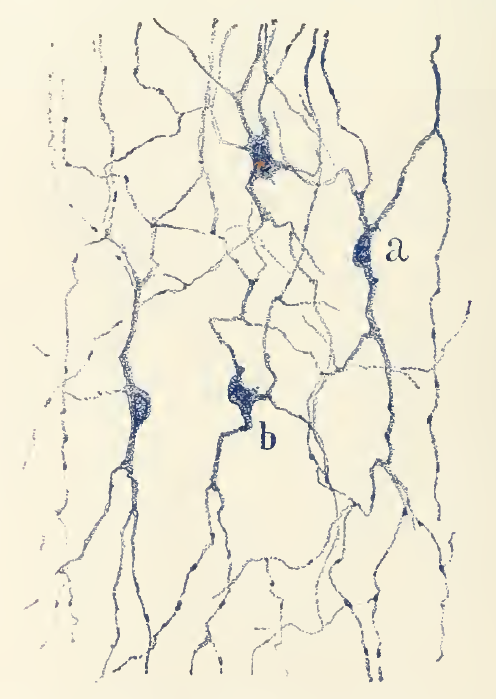
\includegraphics[scale=1]{cajal-nerve-cells.png}
  \caption{Ramón y Cajal 绘制的猫的肠肌层中的神经元细胞。两个神经元细胞体的位置有字母 a 和 b 标出,由细胞体发出的线状的结构是树突和轴突。插图选自\protect\onlinecite{Cajal1909}。}
  \label{figure:cajal-nerve-cells}
\end{figure}

\subsection{神经元}
\label{section:background:neuron}
典型的神经元可以分为三个部分——细胞体、树突和轴突\cite{Gerstner2002}。
图\ref{figure:cajal-neuron-dendrite-axon}中是 Ramón y Cajal 绘制的兔子的大脑中的一个锥体神经元细胞\cite{Cajal1909}。
其中 a 是胞体,b 是树突分支, c 是轴突络,e 是长轴突, l 是多条轴突形成的白质。
功能上,树突是接收信息的结构,胞体是进行信息处理的结构,轴突是输出信息的结构。

\begin{figure}
  \centering
  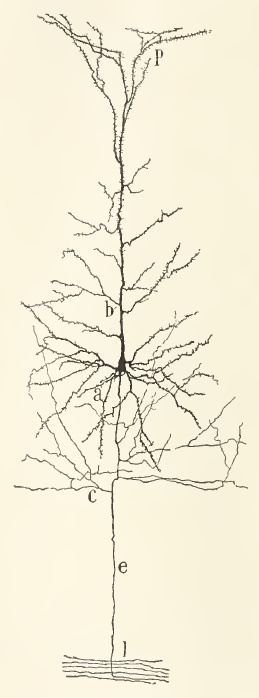
\includegraphics[scale=1]{cajal-neuron-dendrite-axon.png}
  \caption{Ramón y Cajal 绘制的兔子的大脑中的一个金字塔形神经元细胞。 a 是胞体,b 是树突分支, c 是轴突络,e 是长轴突, l 是多条轴突形成的白质。插图选自\protect\onlinecite{Cajal1909}。}
  \label{figure:cajal-neuron-dendrite-axon}
\end{figure}

\subsection{突触}
\label{section:background:synapse}
两个神经元之间连接的结构叫突触。
通常信息通过轴突发出,通过树突接收。
两者可以连接形成突触。

神经元发放动作电位后,对电压敏感的钙离子通道就会打开,钙离子进入细胞内使得突触前神经元内的包含神经递质的囊泡激活,然后与细胞膜融合,将神经递质释放到突触间隙 \cite{bear2007neuroscience,Sudhof2012}。
神经递质经过扩散,与突触后神经元上的神经递质接收器结合,然后经过一系列生化反应,使得突触后神经元上的离子通道打开,产生突触电流 \cite{bear2007neuroscience}。

\section{仿真计算模型}
\label{section:review:simulation-models}
组成神经系统的最基本单元是神经元。
神经元进行信息交流主要靠突触。
要想进行神经系统的仿真计算,首先要建立有效的神经元和突触模型。

\subsection{神经元模型}
\label{section:review:neuron-models}
一种经典的神经元模型是 Hodgkin-Huxley 模型。
模型中包含电压依赖的钠离子通道和电压依赖的钾离子通道等。
当细胞膜电位到达一定范围时,钠离子通道开放率上升,细胞膜电位上升,膜电位的上升又会引起钠离子通道的关闭和钾离子通道的开放率上升,进而使细胞膜电位下降,形成一个动作电位。

加入不同类型的离子通道可以使模型呈现出不同的特性 \cite{Gerstner2002}。
如持续电流刺激下神经元发放频率逐渐降低(发放频率的适应),这一现象可以通过添加钙离子通道和对钙离子浓度敏感的钾离子通道来实现。
这样动作电位产生后,钙离子通道打开,钙离子进入细胞内。
持续发放时,细胞内钙离子浓度积累,使对钙离子浓度敏感的钾离子通道开放率上升,进而使细胞膜电位下降,使得下一个动作电位更难产生 \cite{Gerstner2002}。
Hodgkin-Huxley 模型通过添加离子通道,理论上可以用来模拟各种类型的神经元。
但是由于参数众多,所以定量确定每种离子通道的密度和相关参数所需的数据要求较高。

Izhikevich 分析了各种神经元现象的动力学原理后,提出了简化的 Izhikevich 模型,不模拟离子通道等细节,提高了计算效率,但依然能够通过改变模型参数重现各种神经元动力学现象 \cite{Izhikevich2003,Izhikevich2004}。

\subsection{突触模型}
\label{section:review:synapse-models}
由于大部分突触的现象比较简单,没有神经元动力学那么丰富,所以常用的类型不多。

与 Hodgkin-Huxley 搭配使用时,通常定义一个关于细胞的膜电位的函数,以此作为神经元递质的释放率。
此种模型的突触状态完全依赖于细胞膜电位,不受突触之前释放的影响。

而有研究发现,突触中存在短时程的促进和抑制现象 \cite{Markram1996,Tsodyks1997}。
有些突触在神经元连续发放的情况下,每次释放递质导致的 IPSC 会越来越高,这种称为短时程促进,可能是因为细胞内钙离子积累导致囊泡激活程度提高,进而释放的囊泡增多。
有些突触在神经元连续发放的情况下,每次释放递质导致的 IPSC 会越来越低,这种称为短时程抑制,可能是因为细胞内剩余的可释放囊泡资源减少。
这两种现象合称短时程突触可塑性。
短时程突触可塑性有很多模型,最流行的是 Misha Tsodyks 和 Henry Markram 提出的\cite{Markram1996,Tsodyks1997}。

基于以往人们对神经系统的了解,大部分情况下这些模型就够用了。

\subsection{神经系统中的非同步递质释放}
\label{section:review:asynchronous-neurotransmitter-release-in-the-nervous-system}
在大部分神经元中,递质的释放与动作电位的时间是紧密绑定的,即动作电位之后立刻就会发生递质释放。
然而,在一些神经元中,还存在着另一个释放过程,递质的释放与动作电位没有在时间上紧密绑定,而且释放高度随机,在动作电位结束后很久依然可以存在,这种称为非同步释放。

非同步释放现象在体外培养的神经元中经常发现 \cite{Goda1994,Lau2005}。
在中枢神经系统中,海马区域发现有一类神经元的突触含有很强的非同步释放 \cite{Hefft2005}。

对于非同步释放的生物机制,有多种研究。
有的在斑马鱼的肌肉连接处进行实验,发现非同步释放和同步释放受两种不同的钙离子感受器调控,且同步释放与非同步释的释放量放的在一定时间段内负相关 \cite{Wen2010},意味着它们竞争同一堆囊泡资源。
在中枢神经系统中也发现了不同的钙离子感受器分别调控同步释放和非同步释放 \cite{Sun2007,Bacaj2013}。
也有实验表明中枢神经系统中非同步释放和同步释放竞争同一堆囊泡资源 \cite{Otsu2004}。
细胞内存在两种钙离子感受器也是很早就有发现 \cite{Zengel1977}。

对非同步释放的实验研究有的认为它能增加抑制性 \cite{Medrihan2014},有的认为它能使网络去同步化 \cite{Manseau2010},但网络层面的影响尚不清楚。

有研究发现,在癫痫病人的脑组织中,快速发放神经元的非同步释放比正常人组织中的要强,这可能意味着非同步释放在病理上起着作用,可能是抑制或促进癫痫的发生。

为了研究非同步释放在网络层面的影响,我们先要提出包含非同步释放的理论模型。
然后进行仿真计算,研究它的影响以及分析作用的原理。

\section{论文概要}
\label{section:background:outline}
首先提出包含非同步释放的突触模型,并与实验数据拟合。
然后研究每个参数在单个突触上的作用。
最后在神经元网络层面进行模拟,研究非同步释放对神经元网络行为的影响。
